\section{Prototype}
\label{sec:prototype}
For the purpose of showing some functionality to potential customers of the solution, it was chosen to construct a vertical prototype of the smartphone application.

The prototype only implemented some of the key functionality. The purpose of this is to show a small set of complete functionality. The application was supposed to look like the paper prototype described in \cref{paper_prototype}. Some of the design functionality was not implemented or replaced with a dummy button just to show the potential design.

\begin{figure}[hbtp]
  \centering
  \subfloat[An example search in the prototype.]{
    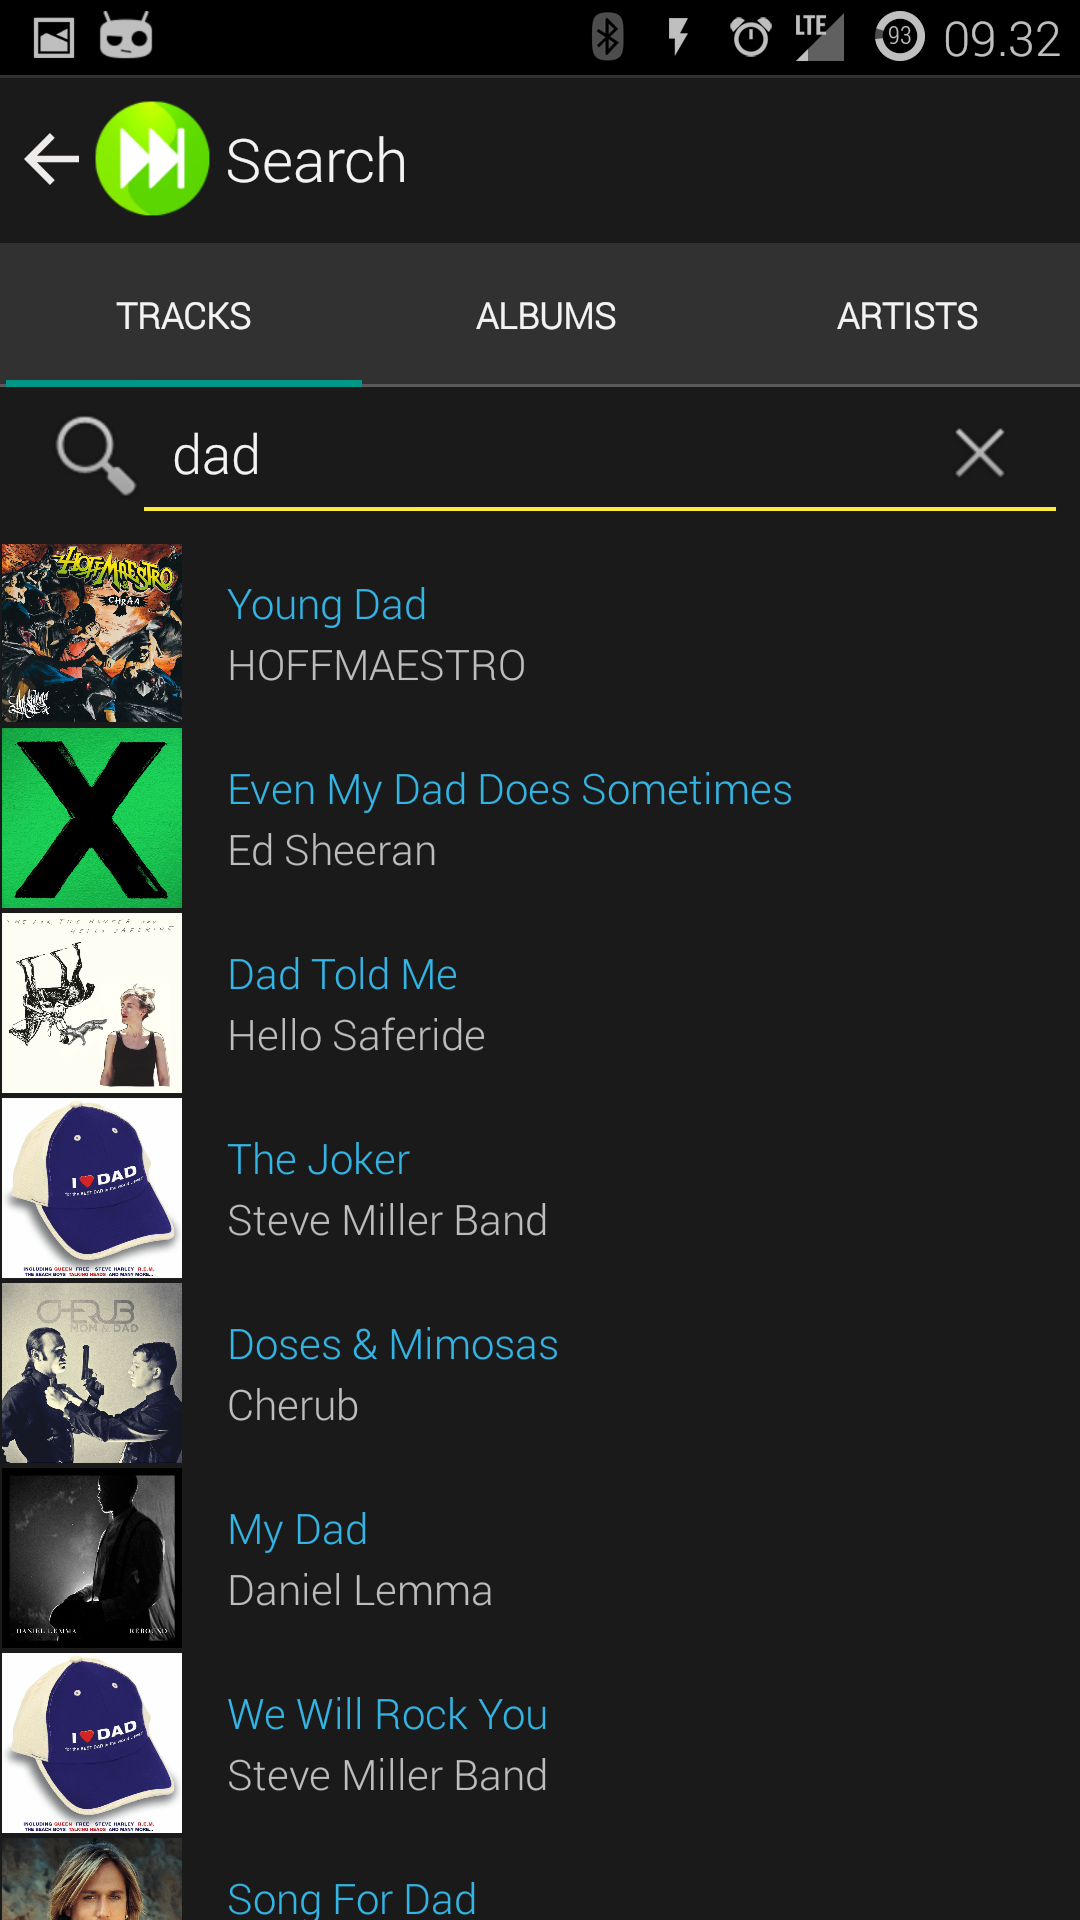
\includegraphics[width=0.5\textwidth]{searchResult}
    \label{fig:searchResult}
  }
  \subfloat[In this early prototype the user still needed to enter the IP manually.]{
    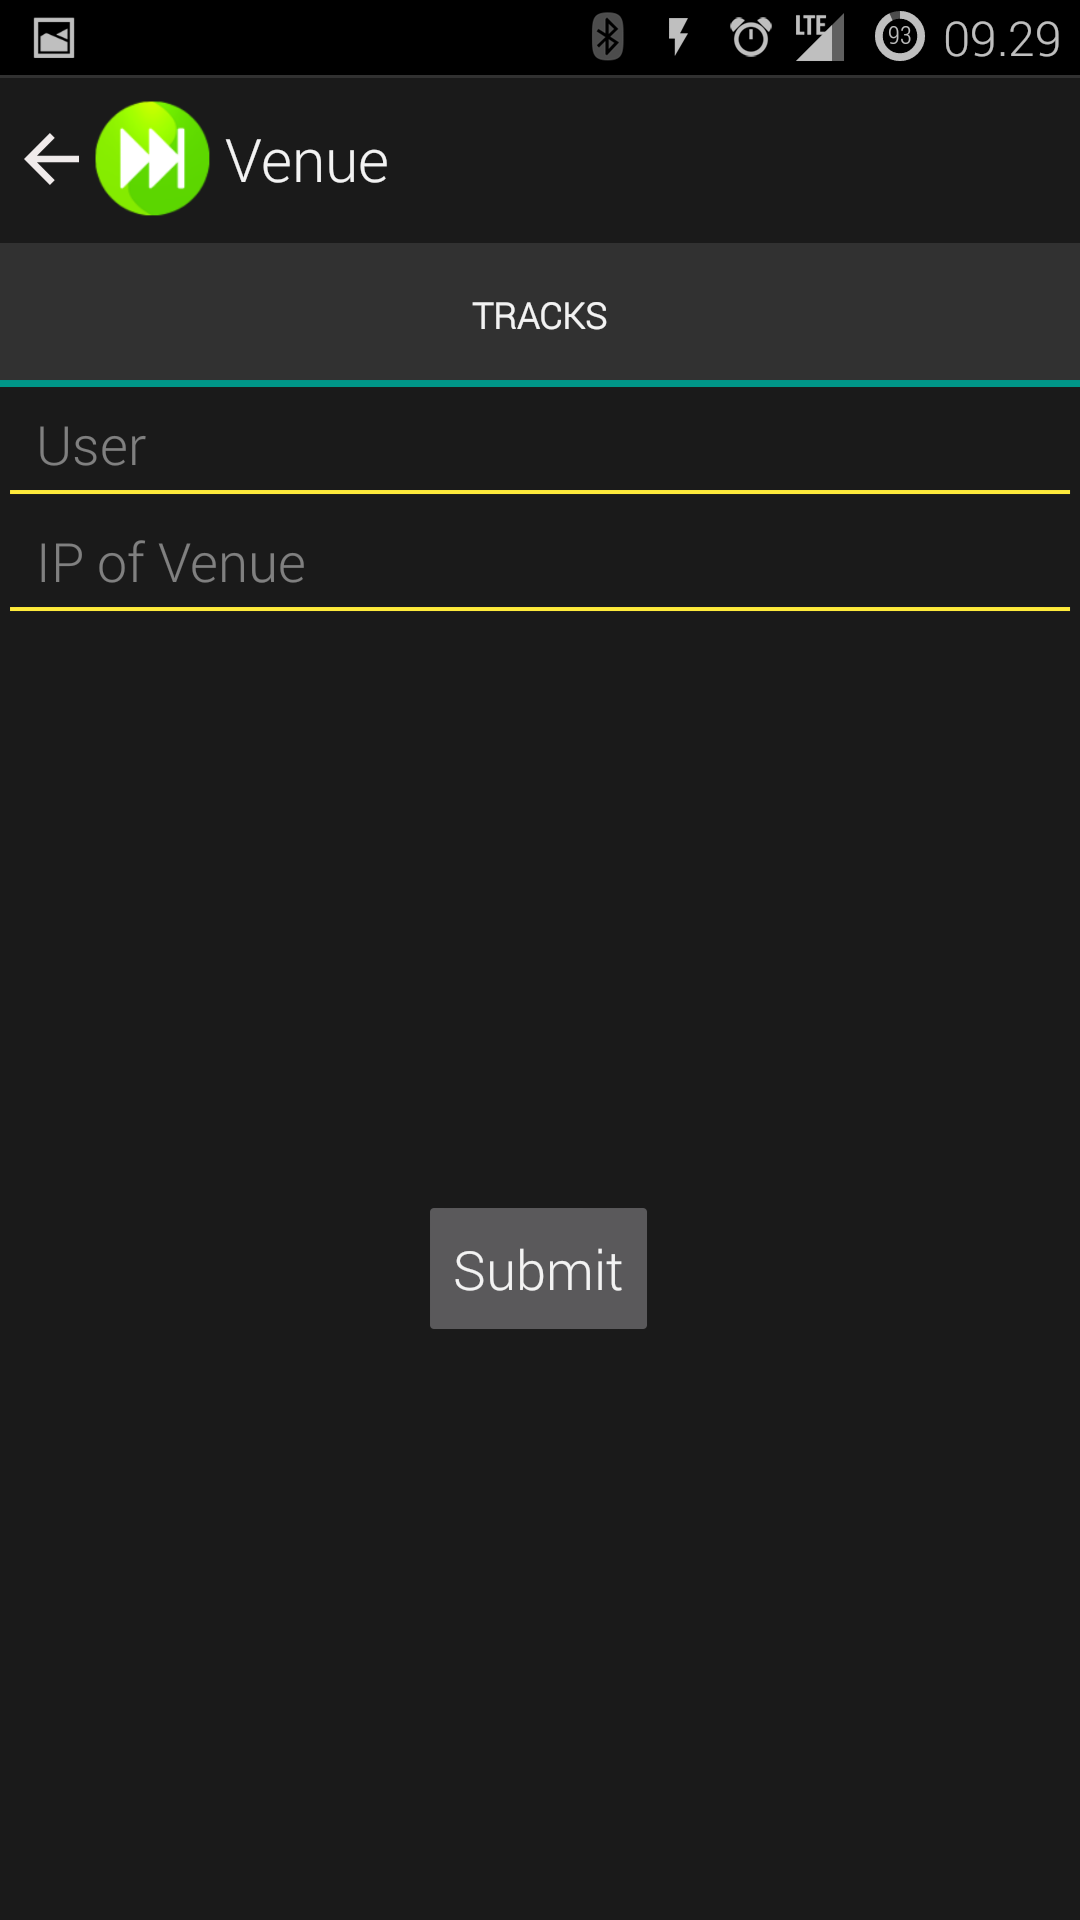
\includegraphics[width=0.5\textwidth]{ipScreen}
    \label{fig:ipScreen}
  }
  \caption{Screenshots from the prototype shown to \enquote{Fabrikken}.}
\end{figure}

\subsection{Vertical Prototype}
\label{sub:vertical_prototype}

The prototype was designed for Android phones, which is one of the mobile platforms that the application is supposed to support. The prototype was supposed to show some of the key functionalities, like the search functionality shown at \cref{fig:searchResult}. The prototype implemented simple functionality that enabled users to vote on a track and send the request to the server. In this prototype the way users checks in at a bar was to type in the IP address of the bar's server and a username, as shown at \cref{fig:ipScreen}. This was an acceptable prototype because the focus was on the playback and search functionality.

\subsection{Collaboration With Industry Partner}
\label{sec:fabrikken}
After the interview with one of the bars from the first set of interviews described in \cref{interviews}, an agreement between the project group and the owner of the bar \enquote{Fabrikken} was made. The owner was willing to test and provide feedback of the application developed in this project. Therefore, another meetup was held with the owner of Fabrikken. A demo of the prototype described in \cref{sec:prototype} was given. It was shown how it was possible to vote on a given track from the smartphone. In response to this demonstration, the owner suggested some additional functionality as listed below.

\begin{itemize}
    \item{The owner would like to access some administration interface on the mobile application, in such a way that it is possible to administer the playlist while standing guard at the door.}
    \item{The owner would like a screen to show the status of the music playback. This could be current and last song played. The currently highest voted song could also be displayed.}
    \item{The owner would like time and date controlled restrictions for the playlist. For example that it is not possible to play the track \enquote{Merry Christmas} from the 26th of December to the 1st of December, the following year.}
    \item{The owner would like to have the drinks menu as a feature in the application.}
    \item{The owner would like to show his offers and events in the application.}
\end{itemize}

Some of the suggested features are not directly associated with any
problems found in the analysis nor described as a concept in the
system definition. In context of this project it is not
necessary to implement these features, but they could and should be
considered in potential further collaborations with the owner of the
bar. The result of the second interview gave additional requirements
for this project, as to the owner wanting to be able to set timed
restrictions for what user can add to the playlist. This concept will
be described in \cref{sec:restrictions}. The owner also wanted to have
a visual output in form of a screen showing the current playlist.
